\chapter{Local Interpretable Model-agnostic Explanations (LIME)}

Local Interpretable Model-agnostic Explanations (LIME) \citep{ribeiro2016whyitrustyou}  is a tool used to visualize the importance of features on the result of a model's prediction.
A score is given to each feature fed to the model, making it possible to understand a black-box model's decision based on its inputs. 

In this chapter, we will discuss how LIME works, how can one use it on image classification models, we will present our implementation of the method and show some experiments done using the technique. 

\section{How it Works}

LIME works by training an interpretable model (\ref{sec:what_is_xai}) to mock the complex \emph{black-box} model over a region of the model's domain.
The underlying idea is that while the model's decision boundary across the entire domain may be complex, it tends to be simpler within smaller, localized regions.

\begin{figure} 
    \centering
    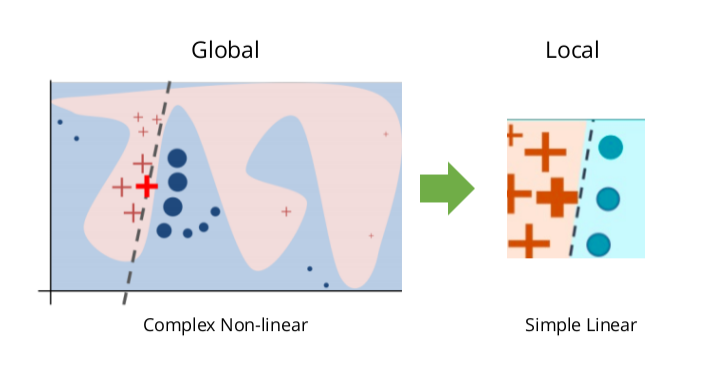
\includegraphics[width=0.5\linewidth]{figuras/lime/lime_regions.png}
    \caption{Smaller regions of model's decion boundary tend to have simple, linear behaviour. Font: C3.ai\footnotemark}
\end{figure}
\footnotetext{https://c3.ai/glossary/data-science/lime-local-interpretable-model-agnostic-explanations/}

To train the interpretable model, a single sample is selected and small perturbations are applied to that data point in order to create a dataset, consisting of the sample image and its perturbations.
Using the dataset, the interpretable model is trained by minimizing the optimization problem bellow:

\begin{equation}
    g^* = \argmin_{g \;\in\; G} \mathcal{L}(f, g, \pi_x) + \Omega(g).
    \label{eq:lime_optimization}  
\end{equation}

Where \(g^*\) is the final trained interpretable model, 
\(G\) is a set of interpretable models, \(f\) is the black-box model, 
\(\Omega\) is a function that maps a model's complexity to a number, with higher complexity yielding higher numbers (Used to penalize complexity in models used to mock the black-box model),
\(\pi_x\) is a function to penalize samples in the dataset "too far" from the original sample \(x\) and
\(\mathcal{L}\) is a cost function to quantify the similarity between the interpretable model's decisions and the complex model's decisions, defined by the expression bellow:

\begin{equation}
    \mathcal{L}(f, g, \pi_x) = \sum_{z, z' \in \; Z} \pi_x(z) (f(z) - g(z'))^2.
    \label{eq:lime_loss}  
\end{equation}

Where \(Z\) is the artificial dataset created from the sample, with datapoints \(z\) - a point with the original model's features, and \(z'\), a data point that represents a transformation applied to those features, like using a subset of inputs or attributes created by \emph{feature engineering}.

% Create a new paragraph to explain better pi_x and how we used it in our implementation.
% Create a new paragraph and talk about what we would do to analyze the new interpretable model to understand the complex model
Because of the huge ammount of variables in a image classification task, directly using an image consisting of hundreds of thousands of pixels in an interpretable model would yield poor results, since analyzing each individual pixel's contribution to a prediction is not well aligned with a human interpretation of image features.
In order to generate more valuable results, a feature engineering technique will be proposed on the next section to model LIME for Image classification tasks. 

\section{LIME on Image Models}

In order to use image models on LIME, one must find a way to transform the features into a more valuable and human-aligned metric. 
To achieve better results, instead of using granular structures such as pixels, we can use \emph{segmentation algorithms} to create \emph{superpixels} of images.
A \emph{superpixel} of an image is a set of pixels in a continuous region of the image. 
For example, the use of the quickshift segmentation algorithm would yield the following superpixel configuration, where the yellow lines represent borders of superpixels:

\newpage

\begin{figure}
    \captionsetup{justification=centering}

    \begin{subfigure}[t]{0.48\textwidth}
        \captionsetup{justification=centering}
        \centering
        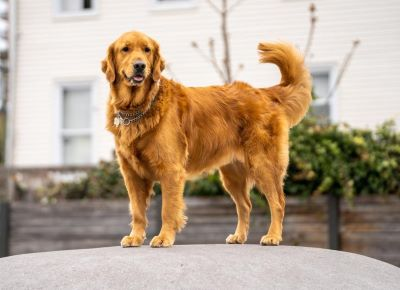
\includegraphics[width=.7\linewidth]{figuras/lime/dog.jpg}
        \caption{Original Image}
    \end{subfigure}
    \hfill
    \begin{subfigure}[t]{0.48\textwidth}
        \captionsetup{justification=centering}
        \centering
        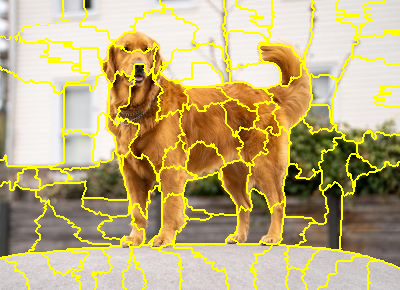
\includegraphics[width=.7\linewidth]{figuras/lime/segmentation_dog.png}
        \caption{Quickshift segmentation}
    \end{subfigure}
    \caption{Superpixel generation using Quickshift}
    \label{fig:superpixel_quickshift}
\end{figure}

To train a model using superpixels, a new dataset would be generated by selecting specific superpixels while discarding others. 
Each data point in this dataset would consist of the original image with certain superpixel regions removed. 
Below is an example of images from this newly created dataset:

\begin{figure}
    \captionsetup{justification=centering}

    \begin{subfigure}[t]{0.31\textwidth}
        \captionsetup{justification=centering}
        \centering
        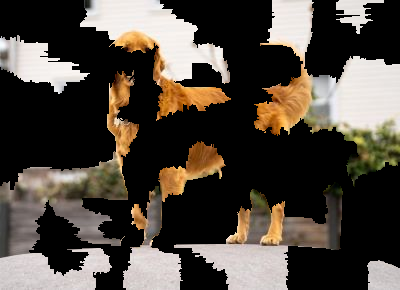
\includegraphics[width=.7\linewidth]{figuras/lime/superpixel_sample0.png}
    \end{subfigure}
    \hfill
    \begin{subfigure}[t]{0.31\textwidth}
        \captionsetup{justification=centering}
        \centering
        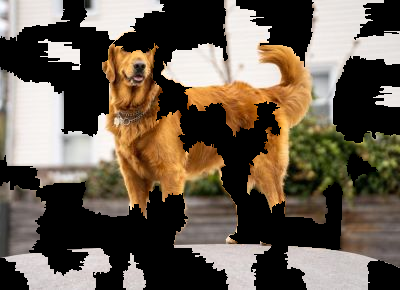
\includegraphics[width=.7\linewidth]{figuras/lime/superpixel_sample1.png}
    \end{subfigure}
    \hfill
    \begin{subfigure}[t]{0.31\textwidth}
        \captionsetup{justification=centering}
        \centering
        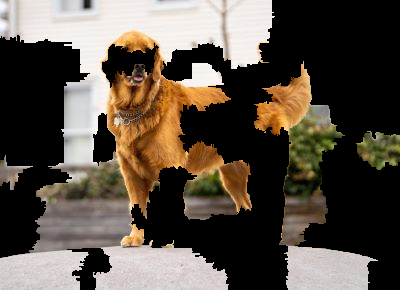
\includegraphics[width=.7\linewidth]{figuras/lime/superpixel_sample2.png}
    \end{subfigure}
    \caption{New dataset samples}
    \label{fig:superpixel_samples}
\end{figure}

These images would then be fed into a complex model to assess the significance of each superpixel in the final prediction. 
Superpixels that play a more crucial role in the model's decision would cause a greater impact on its output.

The interpretable model would be trained using a binary vector \(v \in \{0, 1\}^n\) as input, where each element indicates the presence (1) or absence (0) of a superpixel in the sample, with \(n\) representing the total number of superpixels. 
The output of this interpretable model would be the predicted probability of the desired class.

In the scenario where a Linear Regression model is used, each weight related to each superpixel would represent its importance to the prediction of the desired class.
A high positive weight means that a superpixel positively impacts a probability value, meaning that the portion of the image occupied by the superpixel represents valuable information for the final prediction and should be aligned with the corresponding class, if the model is well trained.

\newpage

An image explanation is shown in image \ref{fig:LIME_vis_image} for the class "Golden Retriever", using a VGG16 model:


\begin{figure}
    \captionsetup{justification=centering}

    \begin{subfigure}[t]{0.48\textwidth}
        \captionsetup{justification=centering}
        \centering
        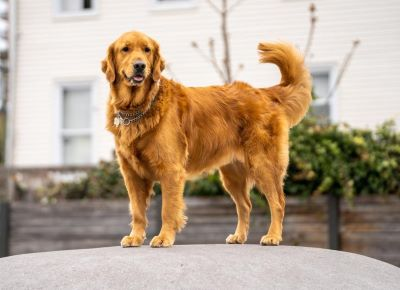
\includegraphics[width=.7\linewidth]{figuras/lime/dog.jpg}
        \caption{Original Image}
    \end{subfigure}
    \hfill
    \begin{subfigure}[t]{0.48\textwidth}
        \captionsetup{justification=centering}
        \centering
        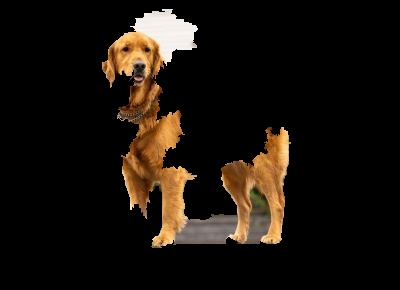
\includegraphics[width=0.5\linewidth]{figuras/lime/lime_dog_sp0.4_dk0.5_nc10.png}
        \caption{LIME Visualization of image}
    \end{subfigure}
    \caption{Visualization of top 15 most important superpixels for "Golden Retriever" ImageNet Class in image}
    \label{fig:LIME_vis_image}
\end{figure}

\section{Implementation}

Using the theory presented in previous sections, an implementation using \href{https://pytorch.org/}{Pytorch} for loading pretrained CNNs, \href{https://scikit-learn.org/stable/}{Scikit-Learn} for Linear models and \href{https://scikit-image.org/}{Scikit-image} for image segmentation using Quickshift.

Our implementation focused on the VGG16 CNN trained on ImageNet, using a Linear Regression model for LIME explanations.
We can load both models with the code bellow:

\begin{program}
    \index{Python}
    \centering

    \begin{lstlisting}[language=Python, style=wider]
        from torchvision.models import vgg16, VGG16_Weights
        from sklearn.linear_model import LinearRegression

        model = vgg16(weights=VGG16_Weights.IMAGENET1K_V1)
        interpretable_model = LinearRegression()
    \end{lstlisting}
\end{program}


The VGG16 model can be seamlessly swapped with other models since LIME operates as a black-box approach, focusing solely on inputs and outputs rather than the model's internal workings.

After the models are loaded, an image to be explained by LIME needs to be loaded. In this example, the image \emph{"dog.jpg"} will be loaded.

\begin{program}
    \index{Python}
    \centering

    \begin{lstlisting}[language=Python, style=wider]
        from PIL import Image
        from torchvision.transforms import ToTensor
        
        to_tensor = ToTensor()
        
        image = Image.open("dog.jpg")
        image = to_tensor(image)
    \end{lstlisting}
\end{program}

Next, we will generate the superpixels of the image using Quickshift, specifying values for \texttt{kernel\_size}, \texttt{max\_dist} and \texttt{ratio}:

\begin{program}
    \index{Python}
    \centering

    \begin{lstlisting}[language=Python, style=wider]
        import torch
        from skimage.segmentation import quickshift
        
        superpixels = torch.tensor(quickshift(
            image.numpy(), 
            kernel_size=kernel_size, 
            max_dist=max_dist, 
            ratio=ratio
        ))
    \end{lstlisting}
\end{program}

With the superpixel mask created, we will generate a new dataset to train our linear model by modifying the original image, chosing a subset of the superpixel set per sample.

\begin{program}
    \index{Python}
    \centering

    \begin{lstlisting}[language=Python, style=wider]
        # create samples tensor
        probability_full_tensor = torch.full((num_samples, num_superpixels), probability)
        samples = torch.bernoulli(probability_full_tensor).to(dtype=torch.int)
        
        # create masks for image to create dataset
    
        image_masks = []
        for sample in samples:
            sample_indexes = torch.nonzero(sample == 1, as_tuple=True)
            mask = torch.isin(superpixels, torch.cat(sample_indexes))
            image_masks.append(mask)
        
        image_masks = torch.stack(image_masks)
        
        # apply each mask to the image, creating a new image per mask
        dataset = image.unsqueeze(0) * image_masks.unsqueeze(1).expand(-1, 3, -1, -1)
    \end{lstlisting}
\end{program}

Now, we extract predictions of the model over each image in the dataset, using a predefined class to visualize called \texttt{explained\_class}:

\begin{program}
    \index{Python}
    \centering

    \begin{lstlisting}[language=Python, style=wider]
        model.eval()
        with torch.no_grad():   # avoid gradient computation
            predictions = model(dataset)[:, explained_class]

    \end{lstlisting}
\end{program}

\newpage

As the final step before training the interpretable model, we compute the distance of each sample in the new dataset from the original image. 
This ensures that the linear model training accounts for the variation between the original image and its modified versions. 

\begin{program}
    \index{Python}
    \centering

    \begin{lstlisting}[language=Python, style=wider]
        cosine_similarity_evaluator = torch.nn.CosineSimilarity(dim=1)
        
        full_ones_samples = torch.ones_like(samples).float()
        cosine_similarity = cosine_similarity_evaluator(full_ones_samples, samples)
        
        sample_weight = torch.sqrt(torch.exp(- cosine_similarity**2 / kernel_samples**2))

    \end{lstlisting}
\end{program}

Here, the sample weight function can be defined as the expression 

\begin{equation}
    \texttt{sample\_weight} = \sqrt{\exp({\texttt{cosine\_similarity}^2 / \texttt{kernel\_samples}^2})}
\end{equation}
where \texttt{cosine\_similarity} is the cosine similarity between the samples tensor and a all-ones tensor and \texttt{kernel\_samples} is a hyperparameter in the interval \((0, 1)\).

Finally, the linear model can now be trained:
\begin{program}
    \index{Python}
    \centering

    \begin{lstlisting}[language=Python, style=wider]
        interpretable_model.fit(
            X=samples,
            y=predictions,
            sample_weight=sample_weight
        )
    \end{lstlisting}
\end{program}

By extracting the interpretable model's weights, we can find the most important regions in the image:

\begin{program}
    \index{Python}
    \centering

    \begin{lstlisting}[language=Python, style=wider]
        from numpy import argsort

        weights = interpretable_model.coef_
        top_features = torch.tensor(argsort(coefs)[-num_selected_weights:])   # select top "num_selected_weights" weights
    
        masked_superpixels = torch.isin(superpixels, top_features)
        visualization_image = image * masked_superpixels
    \end{lstlisting}
\end{program}

Generating a LIME visualization for our desired image.

\section{Experiments} 